%\documentstyle[epsf,twocolumn]{jarticle}       %LaTeX2e仕様
%\documentclass[twocolumn]{jarticle}     %pLaTeX2e仕様(platex.exeの場合)
\documentclass[onecolumn]{ujarticle}   %pLaTeX2e仕様(uplatex.exeの場合)
%%%%%%%%%%%%%%%%%%%%%%%%%%%%%%%%%%%%%%%%%%%%%%%%%%%%%%%%%%%%%%
%%
%%  基本バージョン
%%
%%%%%%%%%%%%%%%%%%%%%%%%%%%%%%%%%%%%%%%%%%%%%%%%%%%%%%%%%%%%%%%%
\setlength{\topmargin}{-45pt}
%\setlength{\oddsidemargin}{0cm}
\setlength{\oddsidemargin}{-7.5mm}
%\setlength{\evensidemargin}{0cm}
\setlength{\textheight}{24.1cm}
%setlength{\textheight}{25cm}
\setlength{\textwidth}{17.4cm}
%\setlength{\textwidth}{172mm}
\setlength{\columnsep}{11mm}

%\kanjiskip=.07zw plus.5pt minus.5pt


% 【節が変わるごとに (1.1)(1.2) … (2.1)(2.2) と数式番号をつけるとき】
%\makeatletter
%\renewcommand{\theequation}{%
%\thesection.\arabic{equation}} %\@addtoreset{equation}{section}
%\makeatother

%\renewcommand{\arraystretch}{0.95} 行間の設定
%%%%%%%%%%%%%%%%%%%%%%%%%%%%%%%%%%%%%%%%%%%%%%%%%%%%%%%%
%\usepackage{graphicx}   %pLaTeX2e仕様(\documentstyle ->\documentclass)
\usepackage[dvipdfmx]{graphicx}
\usepackage{subcaption}
\usepackage{multirow}
\usepackage{amsmath}
\usepackage{url}
\usepackage{ulem}
%%%%%%%%%%%%%%%%%%%%%%%%%%%%%%%%%%%%%%%%%%%%%%%%%%%%%%%%
\begin{document}

	%bibtex用の設定
	%\bibliographystyle{ujarticle}
	% \twocolumn[
	\noindent

	\hspace{1em}
	2020 年 02 月 14 日
	ゼミ資料
	\hfill
	M1 寺内 光

	\vspace{2mm}

	\hrule

	\begin{center}
		{\Large \bf 進捗報告}
	\end{center}


	\hrule
	\vspace{3mm}
	% ]

	% ‚ここから 文章 Start!
	\section{今週やったこと}
	\begin{itemize}{
		\item{画像と台詞の分散表現を取得}
		\item{画像の分散表現のサイズを可変に}
	}
	\end{itemize}

	\subsection{画像と台詞の分散表現を取得}
	Metric Learning に取り組むにあたって画像と台詞の分散表現がどれくらい分離できているのか調べた.表 \ref{fig:t-SNE} に t-SNE によるプロットを示す.いずれも768次元から2次元への圧縮をしている.
	例によって CAE で得られた分散表現はタイトル毎の分離は見られないが,台詞は少し分離できているような気もする...? OL Lunch だけやたら分離できている領域があるのも気になった.解析用のコードを書いたので見せながら.

	\begin{figure}[h]
		\centering
		\begin{subfigure}{0.9\columnwidth}
			\centering
			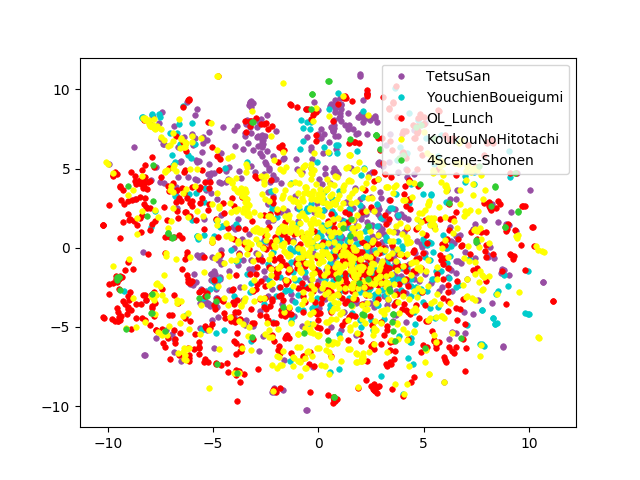
\includegraphics[width=0.9\columnwidth]{data/t_sne_img_80.png}
				\caption{画像の分散表現プロット}
		\end{subfigure}
		\begin{subfigure}{0.9\columnwidth}
			\centering
			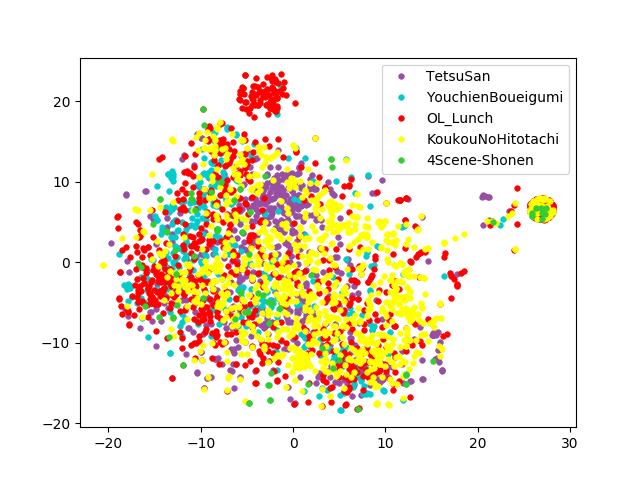
\includegraphics[width=0.9\columnwidth]{data/t_sne_serif_80.png}
				\caption{台詞の分散表現プロット}
		\end{subfigure}
		\caption{t-SNE}
		\label{fig:t-SNE}
	\end{figure}

	\subsection{画像の分散表現のサイズを可変に}
	画像→台詞と台詞→画像のマッチングの識別率に違いがあったため,画像と台詞の分散表現の次元を揃えて再実験した.実装的には CAE のエンコーダの後ろに線形層を挟み中間層の次元を可変にしている(BERTの埋め込み次元768と合わせるため).ちなみにこの処理は keras 時代にもしようとしていたがロスが下がらず画像もほとんど復元できていなかったため断念していた.PyTorch でこの実装を書き,ロスが正常に下がり,解像度は落ちているがしっかりと元画像が復元されていることを確認した.
	図 \ref{fig:loss} に再学習したマッチング実験のロスの遷移を示す.画像と台詞の次元を一致させたが,やはり台詞→画像のマッチング問題が難しいらしい(これはなぜ?).

	\begin{figure}[h]
		\centering
		\begin{subfigure}{0.8\columnwidth}
			\centering
			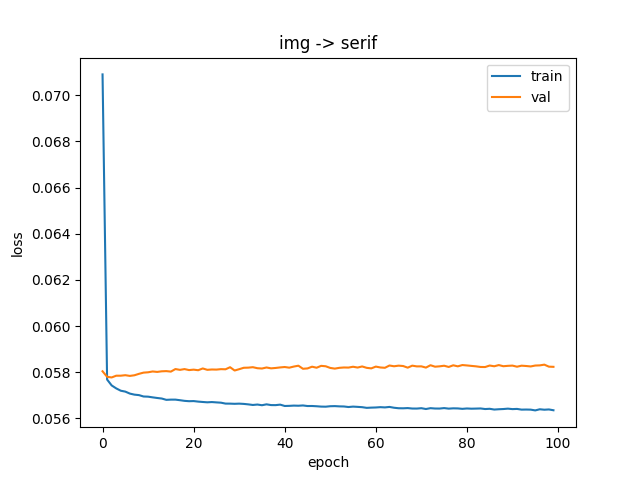
\includegraphics[width=1.0\columnwidth]{data/MLP_imgserif_loss.png}
				\caption{画像→台詞}
		\end{subfigure}
		\begin{subfigure}{0.8\columnwidth}
			\centering
			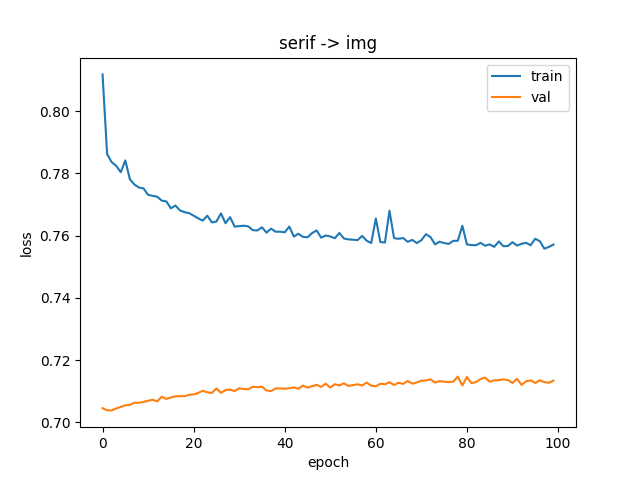
\includegraphics[width=1.0\columnwidth]{data/MLP_serifimg_loss.png}
				\caption{台詞→画像}
		\end{subfigure}
		\caption{ロスの遷移}
		\label{fig:loss}
	\end{figure}

	\section{来週の予定}\noindent
	Metric Learningの知見をためる.かつできれば簡単なモデルを実装.
	%
	% \bibliographystyle{unsrt}
	% \bibliography{2020_01_10_terauchi}

\end{document}
